% \documentclass{report}
% 
% \usepackage{fancyhdr}
\usepackage{fourier-orns}
\usepackage{hyperref}%% To refrence links / jumps
\usepackage{chngcntr} %% For some extra counters numberings
\usepackage[a4paper, right = 0.5in, left = 0.5in,top = 1in , bottom = 1in]{geometry}
\usepackage{etoolbox} %% Provides like a language for advanced customization
\usepackage{datetime} %% For dates of course
\usepackage{lastpage} %% provides pages numbers
\usepackage[sc]{titlesec} %% modify titles
\usepackage{enumerate}
\usepackage{cancel}
\usepackage{tikzsymbols}
\usepackage[dvipsnames]{xcolor}
\usepackage{import}
\usepackage{pdfpages} %% include other pdfs
\usepackage{transparent} %% Transparency
\usepackage{xcolor}  %% Colors
\usepackage[many]{tcolorbox}
\usepackage[framemethod=TikZ]{mdframed}
\usepackage{amsmath,amsfonts,amsthm,amssymb,mathtools}
\usepackage{tikz}
\usepackage{bookmark}
\usepackage{graphicx}
\usepackage{mathpazo}

\usepackage{fontawesome5}

\linespread{1.5}


\titleformat{\chapter}[display]   
{\fontfamily{ppl}\selectfont\huge\color{YellowOrange!80!orange}} % Font style and size 
{\raggedleft\color{purple}\fontsize{70}{0pt}\selectfont\thechapter}   
{-1.5cm}    			                          % Space between the chapter number and title
{
	\begin{tikzpicture}[overlay]
		\node[anchor = west,yshift = 0.2cm,xshift = -1cm] {\fontsize{90}{20} $\int_{}^{} $};
		\node[yshift = 4cm, xshift = 17cm]   {\includegraphics[width = 4cm]{preview0}};
	\end{tikzpicture}
\hspace{1cm}\Huge\raggedright\MakeUppercase}

\titleformat{\section}[block]
{
\fontfamily{ppl}\selectfont\huge\color{YellowOrange!80!orange}
}
{
\color{purple}\fontsize{20}{0pt}\selectfont\thesection 
}
{0cm}
{
	\begin{tikzpicture}[overlay]
		\node[anchor = west,yshift = 0.2cm,xshift = -0.4cm, circle = 1pt] {};
	\end{tikzpicture}
}

\titlespacing*{\section}{0pt}{0.7cm}{1.5cm}


\newcommand{\divider}
{
	\begin{center}
	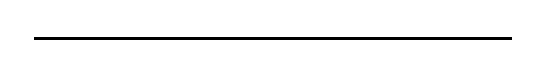
\begin{tikzpicture}
		\draw[thick, black] (0.25*\textwidth, 0) -- (0.75*\textwidth, 0);
		\node[rotate = 360 - 90, xshift = -0.6pt, yshift = 1pt] at (0.25*\textwidth,0){\decotwo};
		\node[rotate = 90, xshift = -0.6pt, yshift = 1pt] at (0.75*\textwidth,0){\decotwo};
	\end{tikzpicture}
	\end{center}
}

\pagestyle{fancy}

\newcommand{\lecday}[1][]
{
    \def\datee{#1}
    \fancyhead[L]{\datee}
}



\newcommand{\signature}
{
	\begin{tikzpicture}[remember picture,overlay]
		\node[fill = YellowOrange!20!white] at ([yshift = 1cm, xshift = -3cm]current page.south east) {\fontsize{10pt}{0pt}{\itshape Kara.$\mathcal{A}$}};
	\end{tikzpicture}
}

\AddToHook{shipout/background}{
  \begin{tikzpicture}[remember picture, overlay]
	  \node[] at ([yshift = 1.5cm,xshift = \textwidth /2 + 0.9cm]current page.south west) {\includegraphics[width = 0.5cm]{preview3}};
	  \node[] at ([yshift = 1.5cm,xshift = - \textwidth /2 - 0.9cm]current page.south east) {\includegraphics[width = 0.5cm]{preview4}};
  \end{tikzpicture}
}



\newtcolorbox[auto counter, number within = section]{remark}[1][]
{
       		title = Remark #1,
		enhanced,
		boxrule = 0pt,
		colback = white,
		breakable,
		arc = 4pt,
		colbacktitle = cyan,
		colback = cyan!5!white,
		segmentation style =
		{
			solid,cyan,thick,
		},
		attach boxed title to top left =
		{
			xshift = 0cm,
		},
		boxed title style =
		{
			boxrule = 0pt,
			sharp corners,
			drop fuzzy shadow = {cyan},
		},
		drop fuzzy shadow = {cyan!80!black},
}

\newtcolorbox[auto counter, number within = section]{theorem}[1][]
{                                      
		title = Theorem \thetcbcounter : #1,
		enhanced, 
		boxrule = 0pt,
		colback = white,
		breakable,
		arc = 4pt,
		colbacktitle = purple,
		colback = purple!5!white,
		segmentation style = 
		{
			solid, purple,thick,
		},
		attach boxed title to top left = 
		{
			xshift = 0cm, 
		},
		boxed title style = 
		{
			boxrule = 0pt,
			sharp corners,
			drop fuzzy shadow = {purple},
		},
		drop fuzzy shadow = {purple!80!black},
}

\newtcolorbox[auto counter, number within = section]{definition}[1][]
{                                      
		title = Definition \thetcbcounter : #1,
		enhanced, 
		boxrule = 0pt,
		colback = white,
		arc = 4pt,
		breakable,
		colbacktitle = YellowOrange!80!black,
		segmentation style = 
		{
			solid, YellowOrange,thick,
		},
		attach boxed title to top left = 
		{
			xshift = 0cm, 
		},
		colback = YellowOrange!5!white,
		boxed title style = 
		{
			boxrule = 0pt,
			sharp corners,
			drop fuzzy shadow = {YellowOrange!80!orange},
		},
		drop fuzzy shadow = {YellowOrange!80!black},
}

\newtcolorbox[auto counter, number within = section]{corollary}[1][]
{                                      
		title = corollary \thetcbcounter : #1,
		enhanced, 
		boxrule = 0pt,
		colback = white,
		arc = 4pt,
		breakable,
		colbacktitle = YellowOrange!80!black,
		segmentation style = 
		{
			solid, YellowOrange,thick,
		},
		attach boxed title to top left = 
		{
			xshift = 0cm, 
		},
		colback = YellowOrange!5!white,
		boxed title style = 
		{
			boxrule = 0pt,
			sharp corners,
			drop fuzzy shadow = {YellowOrange!80!orange},
		},
		drop fuzzy shadow = {YellowOrange!80!black},
}


\newtcolorbox{example}[1][]
{                                      
		title = Example,
		enhanced, 
		boxrule = 0pt,
		colback = white,
		arc = 4pt,
		segmentation style = 
		{
			solid, SpringGreen,thick,
		},
		breakable,
		colback = SpringGreen!5!white,
		colbacktitle = SpringGreen!80!black,
		attach boxed title to top left = 
		{
			xshift = 0cm, 
		},
		boxed title style = 
		{
			boxrule = 0pt,
			sharp corners,
			drop fuzzy shadow = {SpringGreen!80!orange},
		},
		drop fuzzy shadow = {SpringGreen!80!black},
}


\newcommand{\integral}[4]{\int\limits_{#1}^{#2} #4 d#3}
\newcommand{\limit}[3]{\lim\limits_{#1 \rightarrow #2} #3}
\newcommand{\strone}[2]{\left[ \begin{gathered}#1\\ #2\end{gathered} \right] }
\newcommand{\strtwo}[2]{\left\{ \begin{gathered}#1\\ #2\end{gathered} \right\} }
\newcommand{\strthree}[2]{\left\lfloor \begin{gathered}#1\\ #2\end{gathered} \right\rfloor }


\newcommand{\startbf}[1]{\text{\bfseries{#1}}}
\newcommand{\sett}[1]{\left\{ #1 \right\}}
\newcommand{\thesis}[1]{\left( #1 \right)}
\newcommand{\brkt}[1]{\left[ #1 \right]}
\newcommand{\floor}[1]{\left\lfloor #1 \right\rfloor}


\DeclareMathOperator{\img}{im} % Image
\DeclareMathOperator{\Img}{Im} % Image
\DeclareMathOperator{\coker}{coker} % Cokernel
\DeclareMathOperator{\Coker}{Coker} % Cokernel
\DeclareMathOperator{\Ker}{Ker} % Kernel
\DeclareMathOperator{\rank}{rank}
\DeclareMathOperator{\Spec}{Spec} % spectrum
\DeclareMathOperator{\Tr}{Tr} % trace
\DeclareMathOperator{\pr}{pr} % projection
\DeclareMathOperator{\ext}{ext} % extension
\DeclareMathOperator{\pred}{pred} % predecessor
\DeclareMathOperator{\dom}{dom} % domain
\DeclareMathOperator{\ran}{ran} % range
\DeclareMathOperator{\Hom}{Hom} % homomorphism
\DeclareMathOperator{\Mor}{Mor} % morphisms
\DeclareMathOperator{\End}{End} % endomorphism


\newcommand{\lm}{\ensuremath{\lambda}}
\newcommand{\eps}{\ensuremath{\epsilon}}
\newcommand{\veps}{\ensuremath{\varepsilon}}
\newcommand{\al}{\ensuremath{\alpha}}
\newcommand{\bb}{\ensuremath{\beta}}
\newcommand{\cc}{\ensuremath{\gamma}}
\newcommand{\dd}{\ensuremath{\delta}}
\newcommand{\DD}{\ensuremath{\Delta}}
\newcommand{\ff}{\ensuremath{\phi}}
\newcommand{\FF}{\ensuremath{\varphi}}

\newcommand{\RR}{\mathbb{R}}
\newcommand{\RO}{\mathcal{R}}
\newcommand{\EE}{\mathbb{E}}
\newcommand{\CC}{\mathbb{C}}
\newcommand{\RW}{\mathbb{R}^2}
\newcommand{\RT}{\mathbb{R}^3}
\newcommand{\RN}{\mathbb{R}^n}
\newcommand{\DS}{\mathcal{D}}

\newcommand{\KK}{\mathbb{K}}
\newcommand{\KW}{\mathbb{K}^2}
\newcommand{\KT}{\mathbb{K}^3}
\newcommand{\KN}{\mathbb{K}^n}

\newcommand{\NN}{\mathbb{N}}

\newcommand{\PS}{\mathcal{P}}
\newcommand{\AS}{\mathcal{E}}
\newcommand{\FS}{\mathcal{F}}
\newcommand{\LS}{\mathcal{L}}
\newcommand{\MS}{\mathcal{M}}


















\lecday[2025-05-06]

% \begin{document}

\begin{theorem}[Zorn's Lemma]
	Let $X $ be a partially ordered set,
	suppose that every chain in $\mathcal{C}  $ in 
	$X $, that is every totally ordered subset of $X $, has an 
	upper bound in $X$. Then $X $ contains atleast
	one maximal element.
\end{theorem}

% Zorn Lemma  is nice 
%	A = {a,b,c,d,e,f} 
% 	X ⊂ A, x 
	\begin{theorem}[]
	Every vector space has (atleast) a basis.
	\end{theorem}
	\begin{proof}
		Let $E $ be a vector space over some field 
		$\KK $, (not necessarly $\RR  $ or $\CC  $), 
		if $E = \left\{ 0_{E} \right\} $  then 
		$\emptyset  $ is the basis of $E $.
		Now suppose that $E  \neq  \left\{ 0_{E} \right\} $,
		Consider $X $ the set 
		of all linearly independent subsets of 
		$X$ of $E$, we have 
		$X \neq \emptyset  $  because every nonzero 
		vector of $E $ is a linearly independent 
		subset of $E$. we equip $X $ with the 
		partial order of set inclusion 
		\[
			(X, \subset) 
		\]
		for every chain $\mathcal{C}$ of $X$ 
		we claim that the set $\bigcup_{ s \in  \mathcal{C} }^{}  
		S$ is  linearly independent. 
		(i.e. $\in  X $), so 
		$\bigcup_{s \in  \mathcal{S} }^{}  S$ constitutes 
		an upper bound of $\mathcal{C}  $  in $X $, 
		let $n \in \NN $, $\lm_1, \hdots , \lm_{n} \in  \KK $ 
		and $x_1, \hdots , x_{n} \in \bigcup_{S \in  \mathcal{C} }^{} S$   
		such that, 
		\[
		\lm_1 x_1 + \lm_2 x_2 + \hdots + 
		\lm_n x_n  = 0_{E}
		\]
		and show that 
		\[
		\lm_1 = \lm_2 = \hdots  = \lm_n = 0_{\KK}
		\]
		by hypothesis, for all 
		$i \in  \left\{ 1,2, \hdots , n \right\} $  
		there exists $S_{i} \in \mathcal{C} $ such that 
		$x_{i} \in  S_{i} $. Next, since $\mathcal{C}  $  
		is totally ordered, there exists a bijection 
		from $\left\{ 1, \hdots , n \right\} $  
		to $\left\{ 1, \hdots , n  \right\} $  
		such that 
		\[
		S_{\sigma (1)   } \subset 
		S_{\sigma (2)   } \subset 
		\hdots 
		\subset S_{\sigma (n)   }
		\]
		consequently, we have 
		\[
		x_1, \hdots , x_{n} \in  S_{\sigma (n)   } 
		\]
		But since $S_{\sigma (n)   } $  
		is linearly independent, 
		then the equality 
		% @TODO : Look at the proof, and reprove it 
		\[
		\lm_1 x_1 + \lm_2 x_2 + \hdots + \lm_n x_{n} = 0_{E}
		\]                                    
		% @TODO : are collection subsets of X that are totally ordered 
		implies that 
		\[
		\lm_1 = \lm_2 = \hdots = \lm_n = 0_{\KK}
		\]
		as required, our claim is confirmed. \\
		So we can apply the zorn lemma which ensures 
		that $X $ contains atleast one maximal element. 
		Let $B $ be a maximal element of $X $ so 
		$B $ is a linearly indepdent subset 
		of $E $. Next, for every 
		vector $x \in E $, we have either $x \in  B $, 
		thus ( $x \in \left\langle B \right\rangle  $) or 
		$x \notin B $, that is 
		$B \subsetneq  B \cup \left\{ x \right\}$, (implying
		according to the maximality of $B $ in $X $) that 
		\[
		B \cup \left\{ x \right\} \notin X
		\]
		that is,  
		$B \cup \left\{ x \right\} $  is linearly dependent, 
		hence $x \in  \left\langle B \right\rangle   $. 
		So, we have for all $x \in  E $, 
		$x \in  \left\langle B \right\rangle  $. Thus 
		$\left\langle B \right\rangle  = E$, Consequently, 
		$B $ is both linearly independent 
		and spans $E $; that is, $B $ is a a basis of 
		$E $. \\
		Hence the proof is complete.
	\end{proof}
\section{The problem of the extension of continuous linear forms on N.V.S}  
\textbf{Problem 01: } 
Let $E $ and $F $ be two vector spaces over the same field $\KK = \RR  $  or
$\CC$ and let $H $ be a proper subspace of $E$, If 
$ f : H \longrightarrow F $ is a linear mapping from $H $ to $F $ can we extend
it to a linear mapping $ f^{\sim} : E \longrightarrow F$.
\[
\begin{array}{cccc}
      f^{\sim} : &  E  & ^{\pi }\longrightarrow^{H}& F \\

           &    x & \longmapsto     &  f^{\sim}(x) \\ 
\end{array}
\]
\textbf{Answer: Yes!}\\
It sufficies to consider a complementory subspace $G $ of $H $ in $E $, i.e. 
\[
G \oplus H = E
\]
\[
\begin{array}{cccc}
      f^{\sim} : &  E  & \longrightarrow & F \\

           &  x = h+g (h \in  H, g \in  G)  & \longmapsto     & f(h)  \\ 
\end{array}
\]
In other words, we have 
$f^{\sim} = f \circ \pi  $, where $\pi  $ is the projection of $E $ 
into $H $ parallel to $G$  
\[
\begin{array}{cccccc}
	f : &  E  & \longrightarrow^{\pi } & H & \longrightarrow^{f} & F \\

	    &   x=h+g & \longmapsto     & h & \longmapsto & f(h)  \\ 
\end{array}
\]
since $\pi$ is linear then $f^{\sim} = f \circ \pi $  is linear 
and since $\pi (h)  = h (\forall  h \in  H)  $, then 
\[
f^{\sim}_{|H} = 
f 
\]
that is $f^{\sim} $  extends $f $  \\
\textbf{Problem 02: } \\
Now, suppose that $E $ and $F $ are two N.V.S over the same field $\KK = \RR  $ 
or $\CC  $  and let $H $ be a proper normed vector subspace of $E $ and 
$ f : H \longrightarrow F $ \it linear \normalfont and  \it continuous 
\normalfont. Is't possible to extend $f $ to some \it linear \normalfont and   
\it continuous \normalfont mapping 
$ f^{\sim} : E \longrightarrow F $  \\
\textbf{Answer : No, in general ! } \\
% @TODO : Catch up 
Note that the method used to solve \textbf{Problem 01} fails because
the considered projection $\pi $ is in general not continuous. 

% Ist possibel to extend it to the whole space, while garding the 
% continuity, i take a form linear continuous does there exist .
% Banach says that we can do it and we guard the same norm, 
% in other words, we can do it and save the same norm (subordinate norm) 
% thats what hahm banach theorem says in princple 
% thats the theorem we are going to prove. (or we proved.) 
% in principle, thats banach theorem, its more pwoerful
% that extending the continuity, because the borm of the map 
% is saved.

\begin{definition}[]
	Let $E $ be an $\RR$-N.V.S, and 
	$ p : E \longrightarrow \RR  $ be a map, 
	we say that $p $ is sublinear if it satisfies : 
	\begin{enumerate}[(i)]
	\item  
		$p(x+y)   \leq p(x) + p(y)  \quad  \quad 
		(\forall  x,y \in  \RR )$  
	\item  $p( \lm x) = \lm p(x) \quad \quad 
		(\forall  \lm \geq 0, \forall  x \in  E) $  
	\end{enumerate} 
\end{definition}
\begin{theorem}[The Hahn-Banach Theorem]
	Let $E $ be an $\RR  $-vector space and 
	$ p : E \longrightarrow \RR  $ be a \it sublinear \normalfont function.
	Then any lineart form $f $ on a vector subspace of $H $ of $E $ 
	that is dominated above by $p$ has at least one 
	linear extension to all $E $ that is also dominated 
	above by $p $. More explicitly, for every linear 
	form $ f : H \longrightarrow \RR  $ satisfying 
	\[
	f(x)  \leq p(x) \quad \quad 
	(\forall  x \in H) 
	\] 
	 % @TODO : Does the subordinate norm says 
	 %  about the boundendess of the function,
	 % i.e. |||f||| > |||g||| => ? f(x) > g(x)
	 % @TODO: Transfinite recursion ??? 
	there exists a linear form
	 $ f^{\sim} : E  \longrightarrow  \RR $ such that 
	 \[
	 f^{\sim}_{|H} = f \text{ and }  
	 f^{\sim} (x)  \leq  f(x)  \quad  \quad  (\forall  x \in  E) 
	 \] 
	 \begin{proof}
		 Let $H $ be a vector subspace of $E $ 
		 and $ f : H \longrightarrow \RR  $ 
		 be a linear form on $H $  
		 that is dominated above by $p $ since the result of the 
		 theorem is trivial for $H = E $  suppose for the 
		 sequel that $H \neq  E $. \\
		 \textbf{ $1^{st} $ Step } \\
		 let $u \in  E \backslash H $  be fixed
		 we are going to show that there exist a linear 
		 form $ g : H \oplus \RR _{u} \longrightarrow \RR  $, 
		 extending $f $ and satisfying 
		 $g(x)  \leq p(x)  $ for all $x \in  H + \RR_{u}  $, 
		 the determination of such a $g $ is clearly equivalent to 
		 the determination of its value at $u $, that is the determination
		 of $\lm := g(u) \in  \RR   $  so that we have for all
		 $h \in  H $  and all $t \in  \RR  $, 
		 \[
		 g(h + tu)  \leq 
		 p (h+ tu) 
		 \]
		 that is, since $g $ should be linear and extend 
		 $f $, 
		 \[
		 g(h)  + t g(u)  \leq 
		 p(h+ tu) 
		 \]
		 i.e., 
		 \[
		 f(h)   + t\lm \leq 
		 p(h+tu)  \quad \quad 
		 (\forall  h \in  H, \forall  t \in  \RR )  \quad 
		 \quad  (1) 
		 \]
		 since $(1)  $  is obviously 
		 satisfied for $t = 0 $, then we have 
		 \[
			 (1)  \iff 
		 \begin{cases} 
			 f(\frac{1}{t}h)  + 
			 \lm \leq  p(\frac{1}{h} h + u)  \\ 
			f(\frac{1}{t} h) L  +
			\lm \leq 
			-p (- \frac{1}{t} h - u)   
		 \end{cases}
		 \begin{gathered}  
		  \text{ if } t > 0 \quad \quad (2)  \\  
		  \text{ if } t < 0 \quad  \quad (3)  
		 \end{gathered}
		 \]
		 and we have 
		 \begin{align*}
			 (2)  & \iff 
			 \lm \leq  p(x+u) - 
			 f(x)  \quad  \quad  (\forall  x \in  H)  \\
			 (3) & \iff 
			 \lm \geq  f(y)  - p(y-u)  ( \forall  y \in  H) 
		 \end{align*}
		 thus 
		 \begin{align*}
			 (1) & \iff 
			 f(y)  - p(y-u)  \leq 
			 \lm \leq 
			 p(x+u)  - f(x) \quad 
			 \quad  (\forall x,y \in H)  \\
			     & \iff 
			     \sup_{y \in  H}  
			     \left\{ f(y) - p(y-u)   \right\} 
			     \leq \lm \leq 
			     \inf_{x \in  H}  
			     \left\{ 
				     p(x+u)  - f(x) 
			     \right\} \quad \quad (4) 
		 \end{align*}
		 the existence of $\lm $  is then equivalent to 
		 \[
			 \sup_{y \in  H}  
			 \left\{ 
				 f(y)  - p(y-u) 
			 \right\} \leq 
			 \inf_{ x \in  H}  
			 \left\{ p(x+u) - f(x)   \right\} \quad  
			 \quad  (*) 
		 \]
		 Let us show (*), for all $x, y \in H $,
		 we have according to the assumption made on $f $ and
		 $p $, 
		 \begin{align*}
		 f(x) + f(y) = f(x+y)  \leq 
		 p(x+y)  &=  p((y-u) + (x+u)  )  \\
			 & \leq 
			 p(y-u)  + p(x+u) 
		 \end{align*}
		 hence 
		 \[
		 f(y)  - p(y-u)  \leq 
		 p(x+u)  - f(x)  \quad 
		 \quad  (\forall  x,y \in  H) 
		 \]
		 thus, 
		 \[
		 \sup_{y \in  H}  \left\{ 
			 f(y)  - 
			 p(y-u) 
		 \right\} \leq 
		 \inf_{x \in  H}  
		 \left\{ 
			 p(x+u)  - f(x) 
		 \right\}
		 \]
		 confirming $(*)$, Hence the existence of 
		 $\lm $  as required and then the existence of 
		 $g $ as required.
		 \\
		 \textbf{ $2^{nd} $ Step }
		 \\
		 Consider the set $X $ of the pairs 
		 $(F, \FF  )  $,  where $F $ is a subspace of 
		 $E $ containing $H $ and $FF $  is a linear 
		 form on $F $ extending $f $ and satisfying 
		 \[
		 \FF (x)  \leq  p(x) \quad  \quad  (\forall  x \in  F)    
		 \] 
		 Since $(H,f) \in  X  $  then 
		 $X \neq  \emptyset  $, 
		 we equip $X $ with the binary relation $\mathcal{R}$ 
		 defined by 
		 \[
			 (F_1, \FF _{1})   
			 \mathcal{R}  
			 (F_2, \FF _{2})  
			 \iff  F_1 \subset F_2 \text{ and }  
			 \FF_{2|F_{1}} = \FF _{1}
		 \]
		 we easily check that 
		 $ \mathcal{R}  $  is a partial order on $X $.
		 \\
		 Next for every chain $((F_{i}, \FF_{i} ) )_{i \in  I}  $  
		 of $X $, the pair $(F, \FF )  $ given by 
		 \[
		 F = \bigcup_{i \in  I}^{}  
		 F_{i} \quad  
		 \FF (x)  = \FF _{i} (x)  \quad 
		 \quad 
		 (\forall  i \in  I, \forall  x \in  F_{i}) 
		 \]
		 Clearly 


		 The zorn lemma to desire that 
		 $(X, \mathcal{R} )  $  has at least $1$ maximal
		 element $(F^{\sim}, \FF ^{\sim})  $  
		 but if $F^{\sim} \neq E $  
		 and $u \in  E \backslash F^{\sim} $, by the 
		 $1^{st} $  
		 step, we can construct a pair 
		 \[
			 ( F^{\sim} \oplus \RR _{u} , \quad \Psi )  \in 
			 X
		 \]
		 which we strictly greater 



		 Thus $F^{\sim} = E $. So it sufficies to take $f^{\sim} = 
		 \FF ^{\sim}$  to conclude to the resulmt of the theorem:w
		 
	 \end{proof}
\end{theorem} 


% \end{document}
